\Opensolutionfile{ans}[ans/ansTN-NguyenHue029]

\noindent \textbf{PHẦN I. Câu trắc nghiệm có nhiều phương án lựa chọn. Thí sinh trả lời từ câu 1 đến câu 12. Mỗi câu hỏi, thí sinh chỉ chọn một phương án trả lời}
\vspace{0.2cm}

\begin{ex}	\macau{ID: VL12-NH029-C01}Nhiệt nóng chảy riêng của đồng là $1,8 \times 10^{5}\text{ J/kg}$ (trong điều kiện áp suất tiêu chuẩn). Phát biểu nào dưới đây là đúng?
	\choice
	{Khối đồng cần thu nhiệt lượng $1,8 \times 10^{5}\text{ J}$ để hoá lỏng hoàn toàn}
	{Mỗi kilôgam đồng toả ra nhiệt lượng $1,8 \times 10^{5}\text{ J}$ khi hoá lỏng hoàn toàn ở nhiệt độ nóng chảy}
	{Khối đồng sẽ toả ra nhiệt lượng $1,8 \times 10^{5}\text{ J}$ khi nóng chảy hoàn toàn}
	{\True Mỗi kilôgam đồng cần thu nhiệt lượng $1,8 \times 10^{5}\text{ J}$ để hoá lỏng hoàn toàn ở nhiệt độ nóng chảy}
	\loigiai{
		Theo định nghĩa, nhiệt nóng chảy riêng $\lambda = 1,8 \times 10^{5}\text{ J/kg}$ của đồng có nghĩa là mỗi kilôgam đồng cần thu vào một nhiệt lượng bằng đúng $1,8 \times 10^{5}\text{ J}$ để chuyển hoàn toàn từ thể rắn sang thể lỏng ở nhiệt độ nóng chảy tiêu chuẩn}
\end{ex}

\begin{ex}	\macau{ID: VL12-NH029-C02}Khi cọ xát một miếng kim loại lên sàn nhà thì nội năng của miếng kim loại thay đổi bằng cách nào?
	\choice
	{thực hiện lực}
	{\True thực hiện công}
	{truyền nhiệt}
	{truyền nội năng}
	\loigiai{
		Khi cọ xát miếng kim loại lên sàn nhà, lực ma sát trượt sinh công cơ học làm chuyển hóa cơ năng thành nội năng của miếng kim loại, khiến nó nóng lên. Đây là phương thức thay đổi nội năng bằng cách thực hiện công}
\end{ex}

\begin{ex}	\macau{ID: VL12-NH029-C03}Nhiệt độ vào một ngày mùa thu ở Thành phố Huế là $23^\circ\text{C}$. Nhiệt độ đó ứng với bao nhiêu độ theo thang nhiệt độ Kelvin?
	\choice
	{\True $296\text{ K}$}
	{$272\text{ K}$}
	{$305\text{ K}$}
	{$308\text{ K}$}
	\loigiai{
		Áp dụng công thức chuyển đổi giữa hai hệ nhiệt giai bách phân và tuyệt đối:
		$$T\text{ (K)} = t\text{ (}^\circ\text{C)} + 273 = 23 + 273 = 296\text{ K}$$}
\end{ex}

\begin{ex}	\macau{ID: VL12-NH029-C04}Cho hình vẽ dưới đây, trong đó:
	\begin{center}
		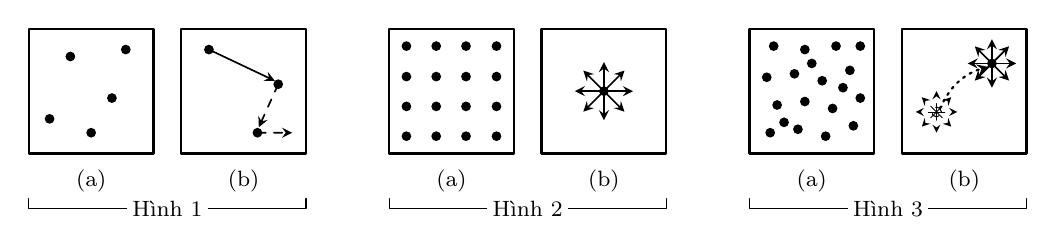
\begin{tikzpicture}[>=stealth, font=\footnotesize, scale=0.88, line cap=round, line join=round]
			% === HINH 1: KHI ===
			\begin{scope}[xshift=0cm]
				\draw[thick] (0,0) rectangle (1.8,1.8);
				\node[below] at (0.9,-0.1) {(a)};
				\foreach \p in {(0.3,0.5), (0.6,1.4), (1.4,1.5), (1.2,0.8), (0.9,0.3)} {
					\fill \p circle (2pt);
				}
				\draw[thick] (2.2,0) rectangle (4.0,1.8);
				\node[below] at (3.1,-0.1) {(b)};
				\coordinate (p1) at (2.6,1.5);
				\coordinate (p2) at (3.6,1.0);
				\coordinate (p3) at (3.3,0.3);
				\fill (p1) circle (2pt);
				\fill (p2) circle (2pt);
				\fill (p3) circle (2pt);
				\draw[->, semithick] (p1) -- (3.55,1.05);
				\draw[->, dashed, semithick] (p2) -- (3.32,0.38);
				\draw[->, dashed, semithick] (p3) -- (3.8,0.3);
				\draw (0,-0.65) -- (0,-0.8) -- (4.0,-0.8) -- (4.0,-0.65);
				\node[fill=white, inner sep=2pt] at (2.0,-0.8) {Hình 1};
			\end{scope}

			% === HINH 2: RAN ===
			\begin{scope}[xshift=5.2cm]
				\draw[thick] (0,0) rectangle (1.8,1.8);
				\node[below] at (0.9,-0.1) {(a)};
				\foreach \x in {0.25, 0.68, 1.11, 1.55} {
					\foreach \y in {0.25, 0.68, 1.11, 1.55} {
						\fill (\x,\y) circle (2pt);
					}
				}
				\draw[thick] (2.2,0) rectangle (4.0,1.8);
				\node[below] at (3.1,-0.1) {(b)};
				\fill (3.1,0.9) circle (2pt);
				\foreach \angle in {0, 45, 90, 135, 180, 225, 270, 315} {
					\draw[->, semithick] (3.1,0.9) -- ++(\angle:0.42);
				}
				\draw (0,-0.65) -- (0,-0.8) -- (4.0,-0.8) -- (4.0,-0.65);
				\node[fill=white, inner sep=2pt] at (2.0,-0.8) {Hình 2};
			\end{scope}

			% === HINH 3: LONG ===
			\begin{scope}[xshift=10.4cm]
				\draw[thick] (0,0) rectangle (1.8,1.8);
				\node[below] at (0.9,-0.1) {(a)};
				\foreach \p in {
					(0.3,0.3), (0.7,0.35), (1.1,0.25), (1.5,0.4),
					(0.4,0.7), (0.8,0.75), (1.2,0.65), (1.6,0.8),
					(0.25,1.1), (0.65,1.15), (1.05,1.05), (1.45,1.2),
					(0.35,1.55), (0.8,1.5), (1.25,1.55), (1.6,1.55),
					(0.5,0.45), (1.35,0.95), (0.9,1.3)
				} {
					\fill \p circle (2pt);
				}
				\draw[thick] (2.2,0) rectangle (4.0,1.8);
				\node[below] at (3.1,-0.1) {(b)};
				\draw[dashed] (2.7,0.6) circle (2pt);
				\foreach \angle in {0, 45, 90, 135, 180, 225, 270, 315} {
					\draw[->, dashed, line width=0.3pt] (2.7,0.6) -- ++(\angle:0.3);
				}
				\draw[->, dotted, thick] (2.75,0.65) to[bend left=25] (3.45,1.25);
				\fill (3.5,1.3) circle (2pt);
				\foreach \angle in {0, 45, 90, 135, 180, 225, 270, 315} {
					\draw[->, semithick] (3.5,1.3) -- ++(\angle:0.35);
				}
				\draw (0,-0.65) -- (0,-0.8) -- (4.0,-0.8) -- (4.0,-0.65);
				\node[fill=white, inner sep=2pt] at (2.0,-0.8) {Hình 3};
			\end{scope}
		\end{tikzpicture}
	\end{center}
	(a) Khoảng cách và sự sắp xếp các phân tử ở các thể khác nhau;\\
	(b) Chuyển động của phân tử ở các thể khác nhau.\\
	Hình cầu là phân tử, mũi tên là hướng chuyển động của phân tử.\\
	Phát biểu nào sau đây là \textbf{không} đúng?
	\choice
	{\True Hình 2b mô tả khoảng cách và sự sắp xếp của các phân tử ở thể lỏng}
	{Quá trình chuyển thể ở Hình 3 sang thể ở Hình 1 khi được đun nóng gọi là sự hóa hơi}
	{Ở hình 2, các phân tử sắp xếp một cách có trật tự, chặt chẽ}
	{Hình 1a mô tả khoảng cách và sự sắp xếp của các phân tử ở thể khí}
	\loigiai{
		Hình 2 mô tả chất ở thể rắn: Hình 2a là cấu trúc trật tự tinh thể của mạng phân tử/nguyên tử ở thể rắn; Hình 2b mô tả dao động nhiệt của phân tử quanh một vị trí cân bằng cố định xác định trong thể rắn, chứ không phải ở thể lỏng. Do đó nhận định A là không đúng}
\end{ex}

\begin{ex}	\macau{ID: VL12-NH029-C05}Nhiệt lượng cần cung cấp để tăng nhiệt độ của vật có khối lượng $m$ (chất làm vật có nhiệt dung riêng $c$) từ nhiệt độ $t_1$ lên tới nhiệt độ $t_2$ được xác định bởi công thức là
	\choice
	{$Q=Lm$}
	{$Q=m\lambda$}
	{$Q=mc(t_2+t_1)$}
	{\True $Q=mc(t_2-t_1)$}
	\loigiai{
		Nhiệt lượng thu vào để làm thay đổi nhiệt độ của một hệ vật chất từ $t_1 \rightarrow t_2$ tuân theo biểu thức: $Q = mc(t_2 - t_1) = mc\Delta t$}
\end{ex}

\begin{ex}	\macau{ID: VL12-NH029-C06}Hình bên dưới là các dụng cụ để đo nhiệt dung riêng của nước. Hãy cho biết dụng cụ số (4) là
	\begin{center}
		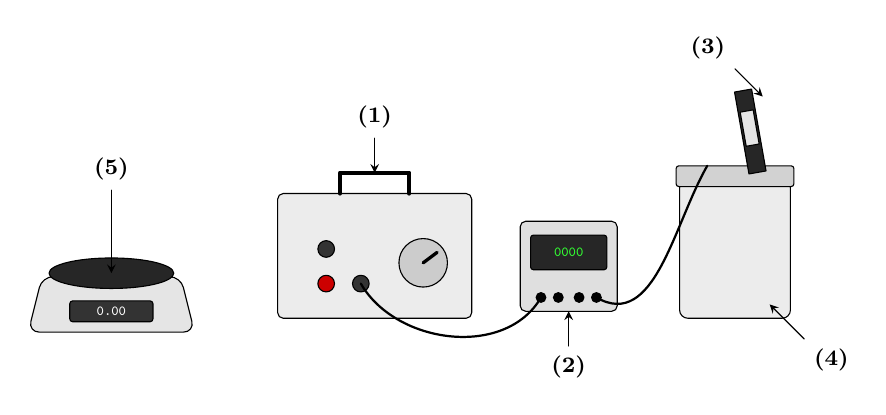
\begin{tikzpicture}[>=stealth, font=\footnotesize, scale=0.88, line cap=round, line join=round]
			% (5) Can dien tu
			\begin{scope}[xshift=0cm, yshift=0cm]
				\draw[fill=gray!20, rounded corners=4pt] (-1.2,0) -- (1.2,0) -- (1.0,0.8) -- (-1.0,0.8) -- cycle;
				\draw[fill=black!85] (0,0.85) ellipse (0.9cm and 0.22cm);
				\draw[fill=black!80, rounded corners=1pt] (-0.6,0.15) rectangle (0.6,0.45);
				\node[text=white, font=\tiny\ttfamily] at (0,0.3) {0.00};
				\coordinate (top5) at (0, 0.85);
			\end{scope}
			
			% (1) Bien the nguon
			\begin{scope}[xshift=3.8cm, yshift=0.2cm]
				\draw[fill=gray!15, rounded corners=2pt] (-1.4,0) rectangle (1.4,1.8);
				\draw[line width=1.5pt, line cap=round] (-0.5,1.8) -- (-0.5,2.1) -- (0.5,2.1) -- (0.5,1.8);
				\draw[fill=gray!40] (0.7,0.8) circle (0.35);
				\draw[line width=1.2pt] (0.7,0.8) -- (0.9,0.95);
				\draw[fill=red!80!black] (-0.7,0.5) circle (0.12);
				\draw[fill=black!80] (-0.2,0.5) circle (0.12);
				\draw[fill=black!80] (-0.7,1.0) circle (0.12);
				\coordinate (power_out1) at (-0.7,0.5);
				\coordinate (power_out2) at (-0.2,0.5);
				\coordinate (top1) at (0, 2.1);
			\end{scope}

			% (2) Oat ke
			\begin{scope}[xshift=6.6cm, yshift=0.3cm]
				\draw[fill=gray!25, rounded corners=2pt] (-0.7,0) rectangle (0.7,1.3);
				\draw[fill=black!85, rounded corners=1pt] (-0.55,0.6) rectangle (0.55,1.1);
				\node[text=green!80!white, font=\tiny\ttfamily] at (0,0.85) {0000};
				\foreach \x in {-0.4, -0.15, 0.15, 0.4} {
					\draw[fill=black] (\x, 0.2) circle (0.07);
				}
				\coordinate (watt_in) at (-0.4, 0.2);
				\coordinate (watt_out) at (0.4, 0.2);
				\coordinate (bot2) at (0, 0);
			\end{scope}

			% (4) Binh nhiet luong ke + (3) Nhiet ke
			\begin{scope}[xshift=9.0cm, yshift=0.2cm]
				\draw[fill=gray!15, rounded corners=3pt] (-0.8,0) rectangle (0.8,2.0);
				\draw[fill=gray!35, rounded corners=1pt] (-0.85,1.9) rectangle (0.85,2.2);
				\coordinate (bot4) at (0.5, 0.2);
				\draw[fill=black!85, rotate around={10:(0.3,2.1)}] (0.2,2.1) rectangle (0.45,3.3);
				\draw[fill=gray!20, rotate around={10:(0.3,2.1)}] (0.23,2.5) rectangle (0.42,3.0);
				\coordinate (top3) at (0.4, 3.2);
				\coordinate (calo_in) at (-0.4, 2.2);
			\end{scope}

			\draw[thick] (power_out2) to[out=-60, in=-120] (watt_in);
			\draw[thick] (watt_out) to[out=-30, in=-120] (calo_in);

			\draw[<-] (top1) -- ++(0, 0.5) node[above] {\textbf{(1)}};
			\draw[<-] (bot2) -- ++(0, -0.5) node[below] {\textbf{(2)}};
			\draw[<-] (top3) -- ++(-0.4, 0.4) node[above left] {\textbf{(3)}};
			\draw[<-] (bot4) -- ++(0.5, -0.5) node[below right] {\textbf{(4)}};
			\draw[<-] (top5) -- ++(0, 1.2) node[above] {\textbf{(5)}};
		\end{tikzpicture}
	\end{center}
	\choice
	{nhiệt kế}
	{cân điện tử}
	{\True nhiệt lượng kế}
	{biến thế nguồn}
	\loigiai{
		Trong sơ đồ bố trí thí nghiệm:
		(1) Biến thế nguồn; (2) Oát kế / đồng hồ đo đa năng; (3) Nhiệt kế điện tử; (4) Nhiệt lượng kế (bình hình trụ có nắp); (5) Cân điện tử. Do đó dụng cụ số (4) là nhiệt lượng kế}
\end{ex}

\begin{ex}	\macau{ID: VL12-NH029-C07}Nhiệt lượng cần thiết để làm cho một kilôgam chất lỏng chuyển đổi pha hoàn toàn từ thể lỏng sang thể khí ở nhiệt độ sôi xác định được gọi là
	\choice
	{nhiệt nóng chảy riêng}
	{nhiệt hoá hơi}
	{nhiệt dung riêng}
	{\True nhiệt hoá hơi riêng}
	\loigiai{
		Theo định nghĩa, lượng nhiệt lượng cần cung cấp để làm cho đúng $1\text{ kg}$ chất lỏng hóa hơi hoàn toàn ở nhiệt độ sôi gọi là nhiệt hóa hơi riêng ($L$, đơn vị $\text{J/kg}$)}
\end{ex}

\begin{ex}	\macau{ID: VL12-NH029-C08}Biết nhiệt nóng chảy riêng của nước đá ở $0^\circ\text{C}$ trong điều kiện áp suất tiêu chuẩn $1\text{ atm}$ là $\lambda = 3,34 \times 10^{5}\text{ J/kg}$. Cung cấp một nhiệt lượng có độ lớn $Q = 5,01 \times 10^{4}\text{ J}$ cho một khối nước đá đang ở $0^\circ\text{C}$ để làm nó nóng chảy hoàn toàn. Giá trị khối lượng $m$ của khối đá là
	\choice
	{$16,7\text{ g}$}
	{$0,167\text{ g}$}
	{$0,15\text{ g}$}
	{\True $150\text{ g}$}
	\loigiai{
		Áp dụng công thức tính khối lượng vật chất chuyển pha nóng chảy:
		$$Q = \lambda \cdot m \Rightarrow m = \frac{Q}{\lambda} = \frac{5,01 \times 10^4}{3,34 \times 10^5} = 0,15\text{ kg} = 150\text{ g}$$}
\end{ex}

\begin{ex}	\macau{ID: VL12-NH029-C09}Chiều cao của cột thủy ngân trong một nhiệt kế thay đổi theo nhiệt độ. Ứng với hai mốc nhiệt độ tiêu chuẩn $0^\circ\text{C}$ và $100^\circ\text{C}$ thì chiều cao cột thủy ngân lần lượt là $2\text{ cm}$ và $22\text{ cm}$. Khi dùng nhiệt kế này đo thân nhiệt của một em bé đang sốt cao, thấy cột thủy ngân dừng ở vạch $9,9\text{ cm}$. Theo thang đo tuyệt đối Kelvin, nhiệt độ cơ thể của em bé là
	\choice
	{$327,0\text{ K}$}
	{\True $312,5\text{ K}$}
	{$321,5\text{ K}$}
	{$305,5\text{ K}$}
	\loigiai{
		- Chiều dài cột thủy ngân tương ứng với dải biến thiên $100^\circ\text{C}$ là: $\Delta \ell = 22 - 2 = 20\text{ cm}$. \\
		- Khi cột thủy ngân cao $9,9\text{ cm}$, khoảng tăng dài từ mốc $0^\circ\text{C}$ là: $\ell_t = 9,9 - 2 = 7,9\text{ cm}$. \\
		- Nhiệt độ cơ thể em bé theo thang Celsius:
		$$t = \frac{\ell_t}{\Delta \ell} \times 100 = \frac{7,9}{20} \times 100 = 39,5^\circ\text{C}$$
		- Quy đổi sang thang tuyệt đối Kelvin: $T = t + 273 = 39,5 + 273 = 312,5\text{ K}$}
\end{ex}

\begin{ex}	\macau{ID: VL12-NH029-C10}Phát biểu nào sau đây là sai khi định tính về các thuộc tính của đại lượng nội năng?
	\choice
	{Nội năng của một vật là dạng năng lượng bao gồm tổng động năng nhiệt của các phân tử và thế năng tương tác giữa chúng}
	{\True Nội năng của một vật là một đại lượng cố định tuyệt đối và không thể biến đổi được}
	{Đơn vị tiêu chuẩn của nội năng trong hệ SI là Jun (J)}
	{Nội năng của một vật phụ thuộc chặt chẽ vào nhiệt độ và thể tích hiện tại của vật}
	\loigiai{
		Nội năng của một vật hoàn toàn có thể biến đổi liên tục thông qua hai phương thức tương tác động lực vĩ mô: thực hiện công hoặc truyền nhiệt. Nhận định B sai}
\end{ex}

\begin{ex}	\macau{ID: VL12-NH029-C11}Chất ở thể rắn có những đặc điểm cấu trúc phân tử nổi bật nào sau đây?
	\choice
	{Các phân tử không giữ được hình dạng cố định vĩ mô}
	{\True Các phân tử có lực liên kết tương tác phân tử vô cùng mạnh mẽ}
	{Các phân tử chuyển động hoàn toàn tự do và hỗn loạn không ngừng về mọi hướng}
	{Các phân tử có khoảng cách rất xa nhau và chiếm toàn bộ thể tích bình chứa}
	\loigiai{
		Chất ở thể rắn đặc trưng bởi lực liên kết phân tử rất mạnh, giữ cho các hạt cấu tử phân bố tuần hoàn chặt chẽ và chỉ dao động quanh vị trí cân bằng cố định}
\end{ex}

\begin{ex}	\macau{ID: VL12-NH029-C12}Khi đề cập đến hai thuật ngữ quá trình "thăng hoa" và quá trình "ngưng kết" trong nhiệt học, ta đang xét đến sự chuyển pha trực tiếp giữa hai thể nào?
	\choice
	{các chất khí hóa lỏng bất kì}
	{thể khí và thể lỏng}
	{thể rắn và thể lỏng}
	{\True thể rắn và thể khí}
	\loigiai{
		- Sự thăng hoa là quá trình chất chuyển pha trực tiếp từ thể rắn sang thể khí/hơi.
		- Sự ngưng kết là quá trình ngược lại, chất chuyển trực tiếp từ thể khí/hơi về thể rắn}
\end{ex}

\Closesolutionfile{ans}

%%%%%%%%%%%%%%%%%%%%%%%%%%%%%%%%%%%%%%%%%%%%%%%%%%%%%%%%%%%%%%%%%%%%%%%%%
% PHẦN II: CÂU TRẮC NGHIỆM ĐÚNG SAI
%%%%%%%%%%%%%%%%%%%%%%%%%%%%%%%%%%%%%%%%%%%%%%%%%%%%%%%%%%%%%%%%%%%%%%%%%
\noindent \textbf{PHẦN II. Câu trắc nghiệm đúng sai. Thí sinh trả lời từ câu 1 đến câu 2. Trong mỗi ý a), b), c), d) ở mỗi câu, thí sinh chọn đúng hoặc sai}
\Opensolutionfile{ans}[ans/ansTF-NguyenHue029]

\begin{ex}	\macau{ID: VL12-NH029-C13}Để xác định nhiệt độ của một lò nung công nghiệp, người ta đặt vào bên trong lò một miếng sắt có khối lượng $75\text{ g}$. Khi miếng sắt đạt trạng thái cân bằng nhiệt bằng với nhiệt độ của lò, người ta nhanh chóng lấy miếng sắt ra thả ngay vào một chiếc nhiệt lượng kế bằng đồng có khối lượng $200\text{ g}$ đang chứa sẵn $500\text{ g}$ nước ở nhiệt độ ổn định $30^\circ\text{C}$. Khi hệ đạt trạng thái cân bằng nhiệt chung, nhiệt kế chỉ vạch $45^\circ\text{C}$. Bỏ qua mọi hao phí nhiệt thất thoát ra môi trường ngoài. Cho biết hằng số nhiệt dung riêng của nước lỏng là $4200\text{ J/(kg}^\circ\text{C)}$, của sắt bằng $478\text{ J/(kg}^\circ\text{C)}$ và của chất làm vỏ nhiệt lượng kế bằng $418\text{ J/(kg}^\circ\text{C)}$.
	\choiceTF[t]
	{Trong tiến trình trao đổi năng lượng trên, tổng nhiệt lượng do miếng sắt tỏa ra bằng đúng lượng nhiệt lượng do riêng khối nước thu vào}
	{Trong quá trình biến đổi trên, bản thân vỏ của nhiệt lượng kế đóng vai trò là vật tỏa nhiệt lượng truyền cấp cho nước lỏng}
	{\True Độ tăng nội năng (lượng nhiệt thu vào) của riêng khối nước lỏng trong bình đạt trị số bằng $31500\text{ J}$}
	{\True Trị số nhiệt độ nội tại của lò nung công nghiệp xấp xỉ bằng $958,6^\circ\text{C}$}
	\loigiai{
		\begin{itemchoice}
			\itemch Vì hệ thu nhiệt bao gồm cả khối nước và bản thân vỏ bình nhiệt lượng kế, nên tổng nhiệt lượng miếng sắt tỏa ra phải bằng tổng nhiệt lượng của nước và nhiệt lượng kế thu vào: $Q_{\text{tỏa}} = Q_{\text{thu nước}} + Q_{\text{thu nlk}}$.
			\itemch Nước và nhiệt lượng kế ban đầu cùng ở $30^\circ\text{C}$, sau đó cùng tăng lên $45^\circ\text{C}$ nhờ nhận nhiệt từ miếng sắt nóng tỏa ra. Do đó vỏ nhiệt lượng kế là vật thu nhiệt, không phải vật tỏa nhiệt.
			\itemch Đổi khối lượng nước: $m_n = 500\text{ g} = 0,5\text{ kg}$. Nhiệt lượng nước thu vào để tăng nhiệt độ từ $30^\circ\text{C} \rightarrow 45^\circ\text{C}$ là:			$$Q_{\text{thu nước}} = m_n \cdot c_n \cdot (t_{\text{cb}} - t_0) = 0,5 \cdot 4200 \cdot (45 - 30) = 31500\text{ J}$$
			Do nước không thực hiện công, độ tăng nội năng $\Delta U_n = Q_{\text{thu nước}} = 31500\text{ J}$.
			\itemch Đổi khối lượng: $m_{\text{sắt}} = 0,075\text{ kg}$; $m_{\text{nlk}} = 0,2\text{ kg}$. Lập phương trình cân bằng nhiệt lượng toàn phần:			$$Q_{\text{tỏa}} = Q_{\text{thu}} \Rightarrow m_{\text{sắt}} \cdot c_{\text{sắt}} \cdot (t_{\text{lò}} - t_{\text{cb}}) = (m_n \cdot c_n + m_{\text{nlk}} \cdot c_{\text{nlk}}) \cdot (t_{\text{cb}} - t_0)$$
			$$0,075 \cdot 478 \cdot (t_{\text{lò}} - 45) = (0,5 \cdot 4200 + 0,2 \cdot 418) \cdot (45 - 30)$$
			$$35,85 \cdot (t_{\text{lò}} - 45) = (2100 + 83,6) \cdot 15 = 2183,6 \cdot 15 = 32754$$
			$$t_{\text{lò}} - 45 = \frac{32754}{35,85} \approx 913,64 \Rightarrow t_{\text{lò}} \approx 958,64^\circ\text{C} \approx 958,6^\circ\text{C}$$
		\end{itemchoice}
	}
\end{ex}

\begin{ex}	\macau{ID: VL12-NH029-C14}Một chiếc nhiệt kế rượu thông dụng được chế tạo với giới hạn đo nhiệt độ an toàn cho phép kéo dài trong dải từ $-115^\circ\text{C}$ cho đến vạch mức $78,5^\circ\text{C}$.
	\choiceTF[t]
	{\True Dóng theo hệ thang đo tuyệt đối Kelvin, dải giới hạn đo tương ứng của chiếc nhiệt kế rượu kể trên kéo dài từ vạch mốc $158\text{ K}$ đến mức $351,5\text{ K}$}
	{\True Chất lỏng rượu được ưu tiên lựa chọn làm môi chất nhiệt kế nhờ vào thuộc tính dãn nở thể tích tương đối đồng đều theo nhiệt độ và có điểm đông đặc cực thấp}
	{\True Chiếc nhiệt kế rượu này hoàn toàn có đủ khả năng kĩ thuật để đo đạc chính xác vạch nhiệt độ môi trường đạt mức tuyệt đối bằng $173\text{ K}$}
	{Ta hoàn toàn có thể dùng chiếc nhiệt kế rượu này phục vụ đo đạc giá trị nhiệt độ sôi của nước lỏng tinh khiết ở điều kiện áp suất tiêu chuẩn $1\text{ atm}$}
	\loigiai{
		\begin{itemchoice}
			\itemch Áp dụng công thức đổi mốc thang đo Kelvin: $T = t + 273$. \\
			- Mốc dưới: $T_{\text{dưới}} = -115 + 273 = 158\text{ K}$. \\
			- Mốc trên: $T_{\text{trên}} = 78,5 + 273 = 351,5\text{ K}$.
			\itemch Rượu dãn nở nhiệt ổn định và đặc biệt có nhiệt độ hóa rắn rất thấp ($-114^\circ\text{C}$), giúp đo được nhiệt độ ở các vùng khí hậu siêu lạnh giá mà nhiệt kế thủy ngân bị đông đặc.
			\itemch Trị số nhiệt độ $173\text{ K}$ tương ứng sang độ Celsius bằng: $t = 173 - 273 = -100^\circ\text{C}$. Trị số này nằm hoàn toàn bên trong dải giới hạn đo cho phép của nhiệt kế [$-115^\circ\text{C}; 78,5^\circ\text{C}$].
			\itemch Ở áp suất tiêu chuẩn nước tinh khiết sôi ở vạch $100^\circ\text{C}$. Trị số này vượt quá giới hạn đo tối đa của nhiệt kế rượu ($78,5^\circ\text{C}$), nếu dùng đo rượu bên trong sẽ sôi làm nổ vỡ nhiệt kế.		\end{itemchoice}
	}
\end{ex}

\Closesolutionfile{ans}

%%%%%%%%%%%%%%%%%%%%%%%%%%%%%%%%%%%%%%%%%%%%%%%%%%%%%%%%%%%%%%%%%%%%%%%%%
% PHẦN III: CÂU TRẮC NGHIỆM TRẢ LỜI NGẮN
%%%%%%%%%%%%%%%%%%%%%%%%%%%%%%%%%%%%%%%%%%%%%%%%%%%%%%%%%%%%%%%%%%%%%%%%%
\noindent \textbf{PHẦN III. Câu trắc nghiệm trả lời ngắn. Thí sinh trả lời từ câu 1 đến câu 4.}
\Opensolutionfile{ans}[ans/ansSA-NguyenHue029]

\begin{ex}	\macau{ID: VL12-NH029-C15}Một hệ vật nặng cơ học có khối lượng $2\text{ kg}$ bắt đầu trượt không vận tốc đầu từ vị trí đỉnh xuống chân của một mặt phẳng nghiêng có chiều dài quỹ đạo quỹ đạo dài $25\text{ m}$, hợp với phương ngang một góc biên độ góc bằng $30^\circ$. Thiết bị cảm biến tốc độ ở chân mặt phẳng nghiêng ghi nhận vận tốc tức thời đạt ngưỡng $5\text{ m/s}$. Tính độ gia tăng nội năng $\Delta U$ của hệ vật trong quá trình chuyển động thẳng trên theo đơn vị Jun (J)? Lấy gia tốc trọng trường $g = 9,8\text{ m/s}^2$ và giả định hoàn toàn không có sự thất thoát nhiệt lượng truyền ra ngoài mặt phẳng nghiêng.

	\par\shortans[oly]{220}
	\loigiai{
		\begin{itemize}
			\item Độ cao hình học ban đầu của đỉnh mặt phẳng nghiêng: $h = \ell \cdot \sin\alpha = 25 \cdot \sin 30^\circ = 12,5\text{ m}$.
			\item Cơ năng ban đầu của vật tại đỉnh dốc (thuần túy là thế năng trọng trường):
			$$W_1 = mgh = 2 \cdot 9,8 \cdot 12,5 = 245\text{ J}$$
			\item Cơ năng cuối của vật tại chân dốc (thuần túy là động năng chuyển động vĩ mô):
			$$W_2 = \frac{1}{2}mv^2 = \frac{1}{2} \cdot 2 \cdot 5^2 = 25\text{ J}$$
			\item Theo định luật bảo toàn năng lượng toàn phần, phần cơ năng vĩ mô bị thất thoát do lực ma sát cản phá sinh công đã chuyển hóa trọn vẹn thành nhiệt năng làm gia tăng nội năng của vật:
			$$\Delta U = W_1 - W_2 = 245 - 25 = 220\text{ J}$$
		\end{itemize}
	}
\end{ex}

\begin{ex}	\macau{ID: VL12-NH029-C16}Một chiếc ấm điện chứa một lượng nước lỏng đang được duy trì đun tới thềm nhiệt độ sôi ổn định $100^\circ\text{C}$ dưới áp suất khí quyển tiêu chuẩn $1\text{ atm}$. Cho biết hằng số ẩn nhiệt hoá hơi riêng của môi chất nước lỏng là $L = 2,26 \times 10^{6}\text{ J/kg}$. Tính lượng nhiệt lượng cần thiết cung cấp để cưỡng bức làm cho khối lượng nước bằng $100\text{ g}$ đang sôi đó hoá thành hơi nước bão hòa hoàn toàn theo đơn vị kilôjun (kJ)?

	\par\shortans[oly]{226}
	\loigiai{
		\begin{itemize}
			\item Quy đổi khối lượng thành phần sang đơn vị kg chuẩn: $m = 100\text{ g} = 0,1\text{ kg}$.
			\item Nhiệt lượng cần cung cấp để phục vụ chuyển pha hóa hơi hoàn toàn lượng nước sôi:
			$$Q = L \cdot m = 2,26 \times 10^6\text{ J/kg} \cdot 0,1\text{ kg} = 226000\text{ J} = 226\text{ kJ}$$
		\end{itemize}
	}
\end{ex}

\begin{ex}	\macau{ID: VL12-NH029-C17}
\immini{
Đồ thị hình bên mô tả sự thay đổi nhiệt độ của nước theo thời gian trong quá trình đun nóng và để nguội. Thời gian xảy ra sự sôi của nước là bao nhiêu phút?
}{
\begin{tikzpicture}[>=stealth, font=\footnotesize, scale=0.68, line cap=round, line join=round]
  \draw[dashed, gray!50, step=1] (0,0) grid (10,5.5);
  \draw[->, thick] (0,0) -- (10.5,0) node[right] {Thời gian (phút)};
  \draw[->, thick] (0,0) -- (0,5.8) node[above] {Nhiệt độ ($^\circ$C)};
  
  \node[left] at (0,0) {$0$};
  \node[left] at (0,1) {$20$};
  \node[left] at (0,2) {$40$};
  \node[left] at (0,3) {$60$};
  \node[left] at (0,4) {$80$};
  \node[left] at (0,5) {$100$};
  
  \node[below] at (1,0) {$2$};
  \node[below] at (2.5,0) {$5$};
  \node[below] at (5,0) {$10$};
  \node[below] at (7.5,0) {$15$};
  \node[below] at (10,0) {$20$};
  
  \coordinate (A) at (0,0);
  \coordinate (B) at (5,5);
  \coordinate (C) at (7,5);
  \coordinate (D) at (10,1.25);
  
  \draw[very thick] (A) -- (B) -- (C) -- (D);
  \node[above left] at (A) {$A$};
  \node[above] at (B) {$B$};
  \node[above] at (C) {$C$};
  \node[right] at (D) {$D$};
\end{tikzpicture}
}

	\par\shortans[oly]{4}
	\loigiai{
		Nhìn vào đồ thị, giai đoạn nước sôi ứng với đoạn nằm ngang $BC$ ở nhiệt độ bão hòa $100^\circ\text{C}$:\\
		- Quá trình sôi bắt đầu tại điểm $B$ ở thời điểm $\tau_1 = 10\text{ phút}$.\\
		- Quá trình sôi kết thúc tại điểm $C$ ở thời điểm $\tau_2 = 14\text{ phút}$.\\
		Thời gian xảy ra sự sôi của nước là:
		$$\Delta \tau = \tau_2 - \tau_1 = 14 - 10 = 4\text{ phút}$$
	}
\end{ex}

\begin{ex}	\macau{ID: VL12-NH029-C18}Tính lượng nhiệt lượng toàn phần theo đơn vị đo kilôjun (kJ) cần thiết cung cấp cho một miếng vật liệu nhôm có khối lượng bằng $100\text{ g}$ đang ở vạch nhiệt độ đầu $20^\circ\text{C}$ để nung nóng nâng nhiệt và làm cho nó hóa lỏng hoàn toàn ở ngưỡng nhiệt độ nóng chảy $659^\circ\text{C}$. Cho biết nhôm có hằng số nhiệt dung riêng bằng $896\text{ J/(kg.K)}$ và hằng số ẩn nhiệt nóng chảy riêng đạt mức $\lambda = 39 \times 10^{4}\text{ J/kg}$. (Kết quả làm tròn lấy đến hàng chữ số đơn vị số nguyên).

	\par\shortans[oly]{96}
	\loigiai{
		\begin{itemize}
			\item Quy đổi khối lượng vật liệu sang kg chuẩn: $m = 100\text{ g} = 0,1\text{ kg}$. Tiến trình gồm 2 giai đoạn:
			- Chặng 1: Thu nhiệt nâng nhiệt độ miếng nhôm từ $20^\circ\text{C} \rightarrow 659^\circ\text{C}$:
			$$Q_1 = m \cdot c \cdot (t_2 - t_1) = 0,1 \cdot 896 \cdot (659 - 20) = 89,6 \cdot 639 = 57254,4\text{ J}$$
			- Chặng 2: Thu ẩn nhiệt chuyển pha hóa lỏng hoàn toàn tại vạch nóng chảy $659^\circ\text{C}$:
			$$Q_2 = m \cdot \lambda = 0,1 \cdot 39 \times 10^4 = 39000\text{ J}$$
			\item Tổng nhiệt lượng toàn phần hệ nhôm thu nhận:
			$$Q = Q_1 + Q_2 = 57254,4 + 39000 = 96254,4\text{ J} \approx 96,25\text{ kJ}$$
			Làm tròn đến chữ số hàng đơn vị theo đúng yêu cầu ta thu được trị số: $96\text{ kJ}$.
		\end{itemize}
	}
\end{ex}

\Closesolutionfile{ans}

%%%%%%%%%%%%%%%%%%%%%%%%%%%%%%%%%%%%%%%%%%%%%%%%%%%%%%%%%%%%%%%%%%%%%%%%%
% PHẦN IV: ĐỀ BÀI CÂU HỎI TỰ LUẬN TÍNH TOÁN (3 ĐIỂM)
%%%%%%%%%%%%%%%%%%%%%%%%%%%%%%%%%%%%%%%%%%%%%%%%%%%%%%%%%%%%%%%%%%%%%%%%%
\noindent \textbf{PHẦN IV. Bài tự luận (3 điểm)}
\vspace{0.2cm}

\begin{ex}	\macau{ID: VL12-NH029-C19}Một lượng chất khí lí tưởng kín hấp thụ nhận vào từ nguồn ngoài một nhiệt lượng có độ lớn bằng $300\text{ J}$ để thực hiện tiến trình dãn nở thể tích và sinh công cơ học đẩy tấm pít-tông dời chỗ, biết chỉ số độ biến thiên nội năng đại số của khối khí ghi nhận được là $\Delta U = +180\text{ J}$. Hãy tính toán xác định độ lớn phần công cơ học do khối chất khí thực hiện giải phóng sinh ra?
	\loigiai{
		- Khối chất khí hấp thụ nhận vào nhiệt lượng từ bên ngoài $\Rightarrow Q = +300\text{ J}$. \\
		- Áp dụng biểu thức hệ thức toán học định luật Nguyên lí I nhiệt động lực học để xác định giá trị công đại số $A$ hệ trao đổi:
		$$\Delta U = Q + A \Rightarrow +180 = 300 + A \Rightarrow A = 180 - 300 = -120\text{ J}$$
		- Trị số công đại số mang dấu âm quy ước ($A = -120\text{ J}$) biểu thị hệ chất khí đã thực hiện sinh công lực đẩy hướng ra ngoại cảnh, với độ lớn phần công cơ học giải phóng đạt trị số bằng:
		$$A' = |A| = 120\text{ J}$$
	}
\end{ex}

\begin{ex}	\macau{ID: VL12-NH029-C20}Một nhà bếp tập thể trường học đang sử dụng một chiếc bếp điện hoạt động đạt chỉ số hiệu suất buồng nhiệt bằng $70\%$ để đun sôi dung tích thể tích $20\text{ lít}$ nước lỏng phục vụ mỗi ngày. Cho biết hằng số nhiệt dung riêng của nước lỏng bằng $4200\text{ J/(kg.K)}$ và khối lượng riêng chất lưu đạt mức $\rho = 1000\text{ kg/m}^3$ (tương đương trị số $1\text{ kg/lít}$). Coi mỗi tháng bếp vận hành liên tục đều đặn trong 30 ngày và nhiệt độ nước cấp đầu vào luôn duy trì ổn định bằng $20^\circ\text{C}$.
	\begin{enumerate}
		\item[a.] Tính lượng điện năng năng lượng toàn phần (theo đơn vị đo tiêu chuẩn Jun) bếp điện tiêu thụ tiêu hao cho mỗi ngày đun nước.
		\item[b.] Tổng cộng trong mỗi tháng, nhà bếp trường học đó phải chi trả tiêu thụ hết bao nhiêu lượng số điện điện năng tính theo đơn vị số điện thương mại kilôgam-giờ ($\text{kW}\cdot\text{h}$)?
	\end{enumerate}
	\loigiai{
		\begin{enumerate}
			\item[a.] Dung tích thể tích nước cần nấu $20\text{ lít}$ tương ứng với khối lượng vật chất bằng $m = 20\text{ kg}$. \\
			Lượng nhiệt lượng có ích cần thiết để đưa khối nước từ điểm mốc đầu tăng nhiệt lên đến vạch điểm sôi $100^\circ\text{C}$ là:
			$$Q_{\text{ích}} = m \cdot c \cdot (t_{\text{sôi}} - t_0) = 20 \cdot 4200 \cdot (100 - 20) = 84000 \cdot 80 = 6720000\text{ J}$$
			Do hiệu suất truyền nhiệt của bếp điện chỉ đạt mức $H = 70\% = 0,7$, lượng điện năng năng lượng toàn phần bếp bắt buộc phải tiêu thụ rút từ mạng điện cho mỗi ngày đun là:
			$$W_{\text{ngày}} = \frac{Q_{\text{ích}}}{H} = \frac{6720000\text{ J}}{0,7} = 9600000\text{ J} = 9,6 \cdot 10^6\text{ J}$$
			\item[b.] Thực hiện tính tổng lượng điện năng năng lượng tiêu thụ của nhà bếp tích lũy trong cả tháng kéo dài 30 ngày hoạt động liên tục:
			$$W_{\text{tháng}} = 30 \cdot W_{\text{ngày}} = 30 \cdot 9600000\text{ J} = 288000000\text{ J} = 2,88 \cdot 10^8\text{ J}$$
			Thực hiện quy đổi giá trị năng lượng tổng tìm được sang đơn vị đo điện năng thương mại tiêu chuẩn số điện ($\text{kW}\cdot\text{h}$) theo quy tắc chuyển đổi hệ số ($1\text{ kW}\cdot\text{h} = 3,6 \cdot 10^6\text{ J}$):
			$$E_{\text{tháng}} = \frac{288000000\text{ J}}{3,6 \cdot 10^6\text{ J/kW}\cdot\text{h}} = 80\text{ kW}\cdot\text{h} \quad \text{(Tương đương mức tiêu thụ bằng 80 số điện)}$$
		\end{enumerate}
	}
\end{ex}

\begin{ex}	\macau{ID: VL12-NH029-C21}Người ta sử dụng một chiếc ấm điện hoạt động ở điều kiện ổn định với công suất tiêu thụ định mức bằng $P = 1000\text{ W}$ để đun một lượng khối lượng $m = 300\text{ g}$ nước lỏng đang ở vạch nhiệt độ ban đầu $20^\circ\text{C}$ tiến đến điểm sôi bão hòa $100^\circ\text{C}$ dưới áp suất tiêu chuẩn. Cho biết các hằng số kĩ thuật: nhiệt dung riêng của nước lỏng bằng $4200\text{ J/(kg.K)}$ và hằng số ẩn nhiệt hoá hơi riêng bằng $2,26 \times 10^{6}\text{ J/kg}$. Giả định hệ lý tưởng bỏ qua mọi hao phí thất thoát nhiệt lượng truyền ra ngoài vỏ ấm và không khí. Nếu chiếc ấm điện được duy trì cắm điện bật liên tục trong khoảng thời gian dài trọn vẹn đúng $\tau = 2,5\text{ phút}$ tính từ thời điểm khởi động máy, hãy tính toán xác định lượng khối lượng nước lỏng thực tế còn dư dính lại an toàn bên bên trong ấm bằng bao nhiêu gam?
	\loigiai{
		\begin{itemize}
			\item Quy đổi đồng bộ đơn vị đo các thông số đầu vào sang hệ SI: khối lượng nước $m = 0,3\text{ kg}$; khoảng thời gian đun $\tau = 2,5\text{ phút} = 2,5 \cdot 60 = 150\text{ giây}$.
			\item Tổng năng lượng nhiệt lượng toàn phần do dòng điện chạy qua ấm điện cung cấp giải phóng ra trong suốt 150 giây đun đạt mức:
			$$Q_{\text{tổng}} = P \cdot \tau = 1000\text{ W} \cdot 150\text{ s} = 150000\text{ J}$$
			\item Lượng nhiệt lượng tiêu hao cần thiết phục vụ cho giai đoạn đầu nâng nhiệt toàn bộ khối nước từ thềm $20^\circ\text{C}$ đạt tiến sát đến thềm điểm sôi $100^\circ\text{C}$:
			$$Q_1 = m \cdot c \cdot (t_{\text{sôi}} - t_0) = 0,3 \cdot 4200 \cdot (100 - 20) = 1260 \cdot 80 = 100800\text{ J}$$
			\item Nhận thấy $Q_{\text{tổng}} = 150000\text{ J} > Q_1 = 100800\text{ J}$, chứng tỏ lượng năng lượng dư thừa tiếp tục làm nước sôi bùng lên bốc hơi chuyển pha dời hệ. Lượng năng lượng dư dùng cấp cho quá trình hóa hơi bão hòa bằng hiệu số:
			$$Q_2 = Q_{\text{tổng}} - Q_1 = 150000 - 100800 = 49200\text{ J}$$
			\item Khối lượng phần hơi nước bão hòa đã bứt phá bốc hơi bay thoát đi ra ngoài không khí:
			$$\Delta m = \frac{Q_2}{L} = \frac{49200\text{ J}}{2,26 \times 10^6\text{ J/kg}} \approx 0,02177\text{ kg} \approx 21,77\text{ g}$$
			\item Lượng khối lượng nước lỏng thực tế còn dư dính lại an toàn bên bên trong ấm siêu tốc:
			$$m_{\text{còn}} = m - \Delta m = 300\text{ g} - 21,77\text{ g} \approx 278,23\text{ g}$$
		\end{itemize}
	}
\end{ex}

\Closesolutionfile{ans}

\newpage
%%%%%%%%%%%%%%%%%%%%%%%%%%%%%%%%%%%%%%%%%%%%%%%%%%%%%%%%%%%%%%%%%%%%%%%%%
% KHUNG ĐÁP ÁN BẢNG TỰ ĐỘNG IN KẾT XUẤT CỦA HỆ THỐNG
%%%%%%%%%%%%%%%%%%%%%%%%%%%%%%%%%%%%%%%%%%%%%%%%%%%%%%%%%%%%%%%%%%%%%%%%%
\begin{center} \textbf{BẢNG ĐÁP ÁN THAM KHẢO LỚP 12 --- MÃ ĐỀ \thedeso} \end{center}

\noindent \textbf{Phần I (Câu hỏi trắc nghiệm nhiều phương án lựa chọn):}